\captionsetup{justification=centering,margin=0cm}
\label{cap:atividade1}  % Forma de referenciar o capítulo no comando \ref

%inicio do capitulo
\chapter[Atividade 1: ENTENDENDO IMAGENS VETORIAIS E \textit{BITMAPS}]{Atividade 1: ENTENDENDO IMAGENS VETORIAIS E \textit{BITMAPS}}

Como é sabido, pode-se dividir as imagens em dois tipos distintos: imagens vetoriais e imagens \textit{bitmap}. Ambas possuem as suas características e utilidades e essa seção busca explicitar essas diferenças.

\section{Conceituando imagens \textit{bitmaps} e vetoriais}

A priori, pode-se entender uma imagem em \textit{bitmap} como uma matriz com "I" linhas, "J" colunas e "K" canais. Cada elemento dessa matriz é um \textit{pixel}, unidade fundamental de composição de imagens, composto por um vetor "K" que varia de acordo com o formato do arquivo.

\hspace{1.5 cm} Uma imagem vetorial, por outro lado, consiste em uma fórmula matemática que gera uma imagem. Essa função recebe como parâmetro a escala utilizada, então o computador renderiza a imagem a partir desses parâmetros e dessa função. Inclusive, esse PDF possui fontes vetoriais!

\hspace{1.5 cm} Como pode-se perceber, ambas as imagens são feitas de forma diferentes, logo é de se esperar que elas possuam características distintas. No geral, imagens em \textit{bitmap} são mais indicadas em situações onde é preciso muitas informações. Fotos do mundo real, por exemplo, são feitas em \textit{bitmap}; o problema disso é que além delas serem costumeiramente mais "pesadas" que imagens vetoriais, a ampliação da imagem implica na redução da qualidade da imagem. Já imagens vetoriais, por serem fórmulas, costumam ser mais leves (mas depende da quantidade de detalhes que a imagem busca ter) e o zoom nela não perde qualidade.

\subsection{SVG, Composição Interna}
Existem muitos tipos de arquivos de imagem. O tipo escolhido para fazer essa atividade é o SVG (\textit{Scalable Vector Graphics}) muito utilizado no contexto do desenvolvimento \textit{web}. Antes de analisar as imagens, deve-se compreender a sua estrutura. Para fazer essa análise, utilizou-se o editor de texto "Notepad++".

\hspace{1.5 cm} Assim como muitos outros arquivos de imagem, o SVG inicia com um cabeçalho (\textit{header}) que contém algumas informações básicas sobre ele. Depois, uma série de comando são utilizados, seguindo uma sintaxe semelhante à nossa linguagem de marcação favorita, o HTML5 (Linguagem de Marcação de Hipertexto). Curiosos, decidimos fazer algumas pesquisas e descobrimos que existe uma \textit{tag} no HTML5 chamada svg. Ou seja, basta "ligar o tico no teco", uma imagem SVG nada mais é do que uma composição da tag svg do HTML, expandida para um arquivo separado na composição da página, justificando o seu vasto uso no contexto web.

\section{Percepções Sobre Imagens Vetoriais}
Utilizou-se 5 imagens para fazer observações sobre esse tipo de composição. Como esperado o zoom na imagem não influencia na qualidade. Ademais, como esperado, as imagens não possuem textura. Se for analisado com cautela, pode-se perceber que conceitos como luz e sombra são aplicados, assim como variações de tons e degradês. Contudo, por se tratar de um desenho essencialmente, as imagens possuem cores sólidas preenchendo totalmente o espaço. Isso não costuma ser um problema, mas se observar a Imagem \ref{fig:carro} você há de notar como é esquisito esse carro.

\begin{figure}[h!]
    \centering
    \caption{Carro no formato SVG}
    \label{fig:carro}
    
    \includesvg[scale=0.1]{Documeto/1-ElementosTextuais/1-Desenvolvimento/imagens-atividade1/NewTux.svg}

    \fonteElementoGrafico{Fornecido pelo Professor}
    
\end{figure}

\hspace{1.5 cm} Acreditamos que essa sensação aconteça nessa figura em particular por dois motivos. O primeiro é que essa imagem propõe-se a parecer mais realista, trazendo muito a percepção de luz e sombra, o que faz o cérebro buscar por outras informações que não existem. A segunda é porque a imagem traz um carro, objeto tão familiarizado por nós que nos força a buscar informações mais realistas nele. 

\section{Comparando Imagens Vetoriais e \textit{Bitmaps}}
Já foi explicado a diferença entre os dois tipos de imagem. Agora, vamos explicitar a diferença entre elas. Abaixo, seguem as Imagens \ref{fig:carro_png} e \ref{fig:carro_SVG}.

\begin{figure}[h!]
    \centering
    \caption{Carro no formato PNG}
    \label{fig:carro_png}
    
    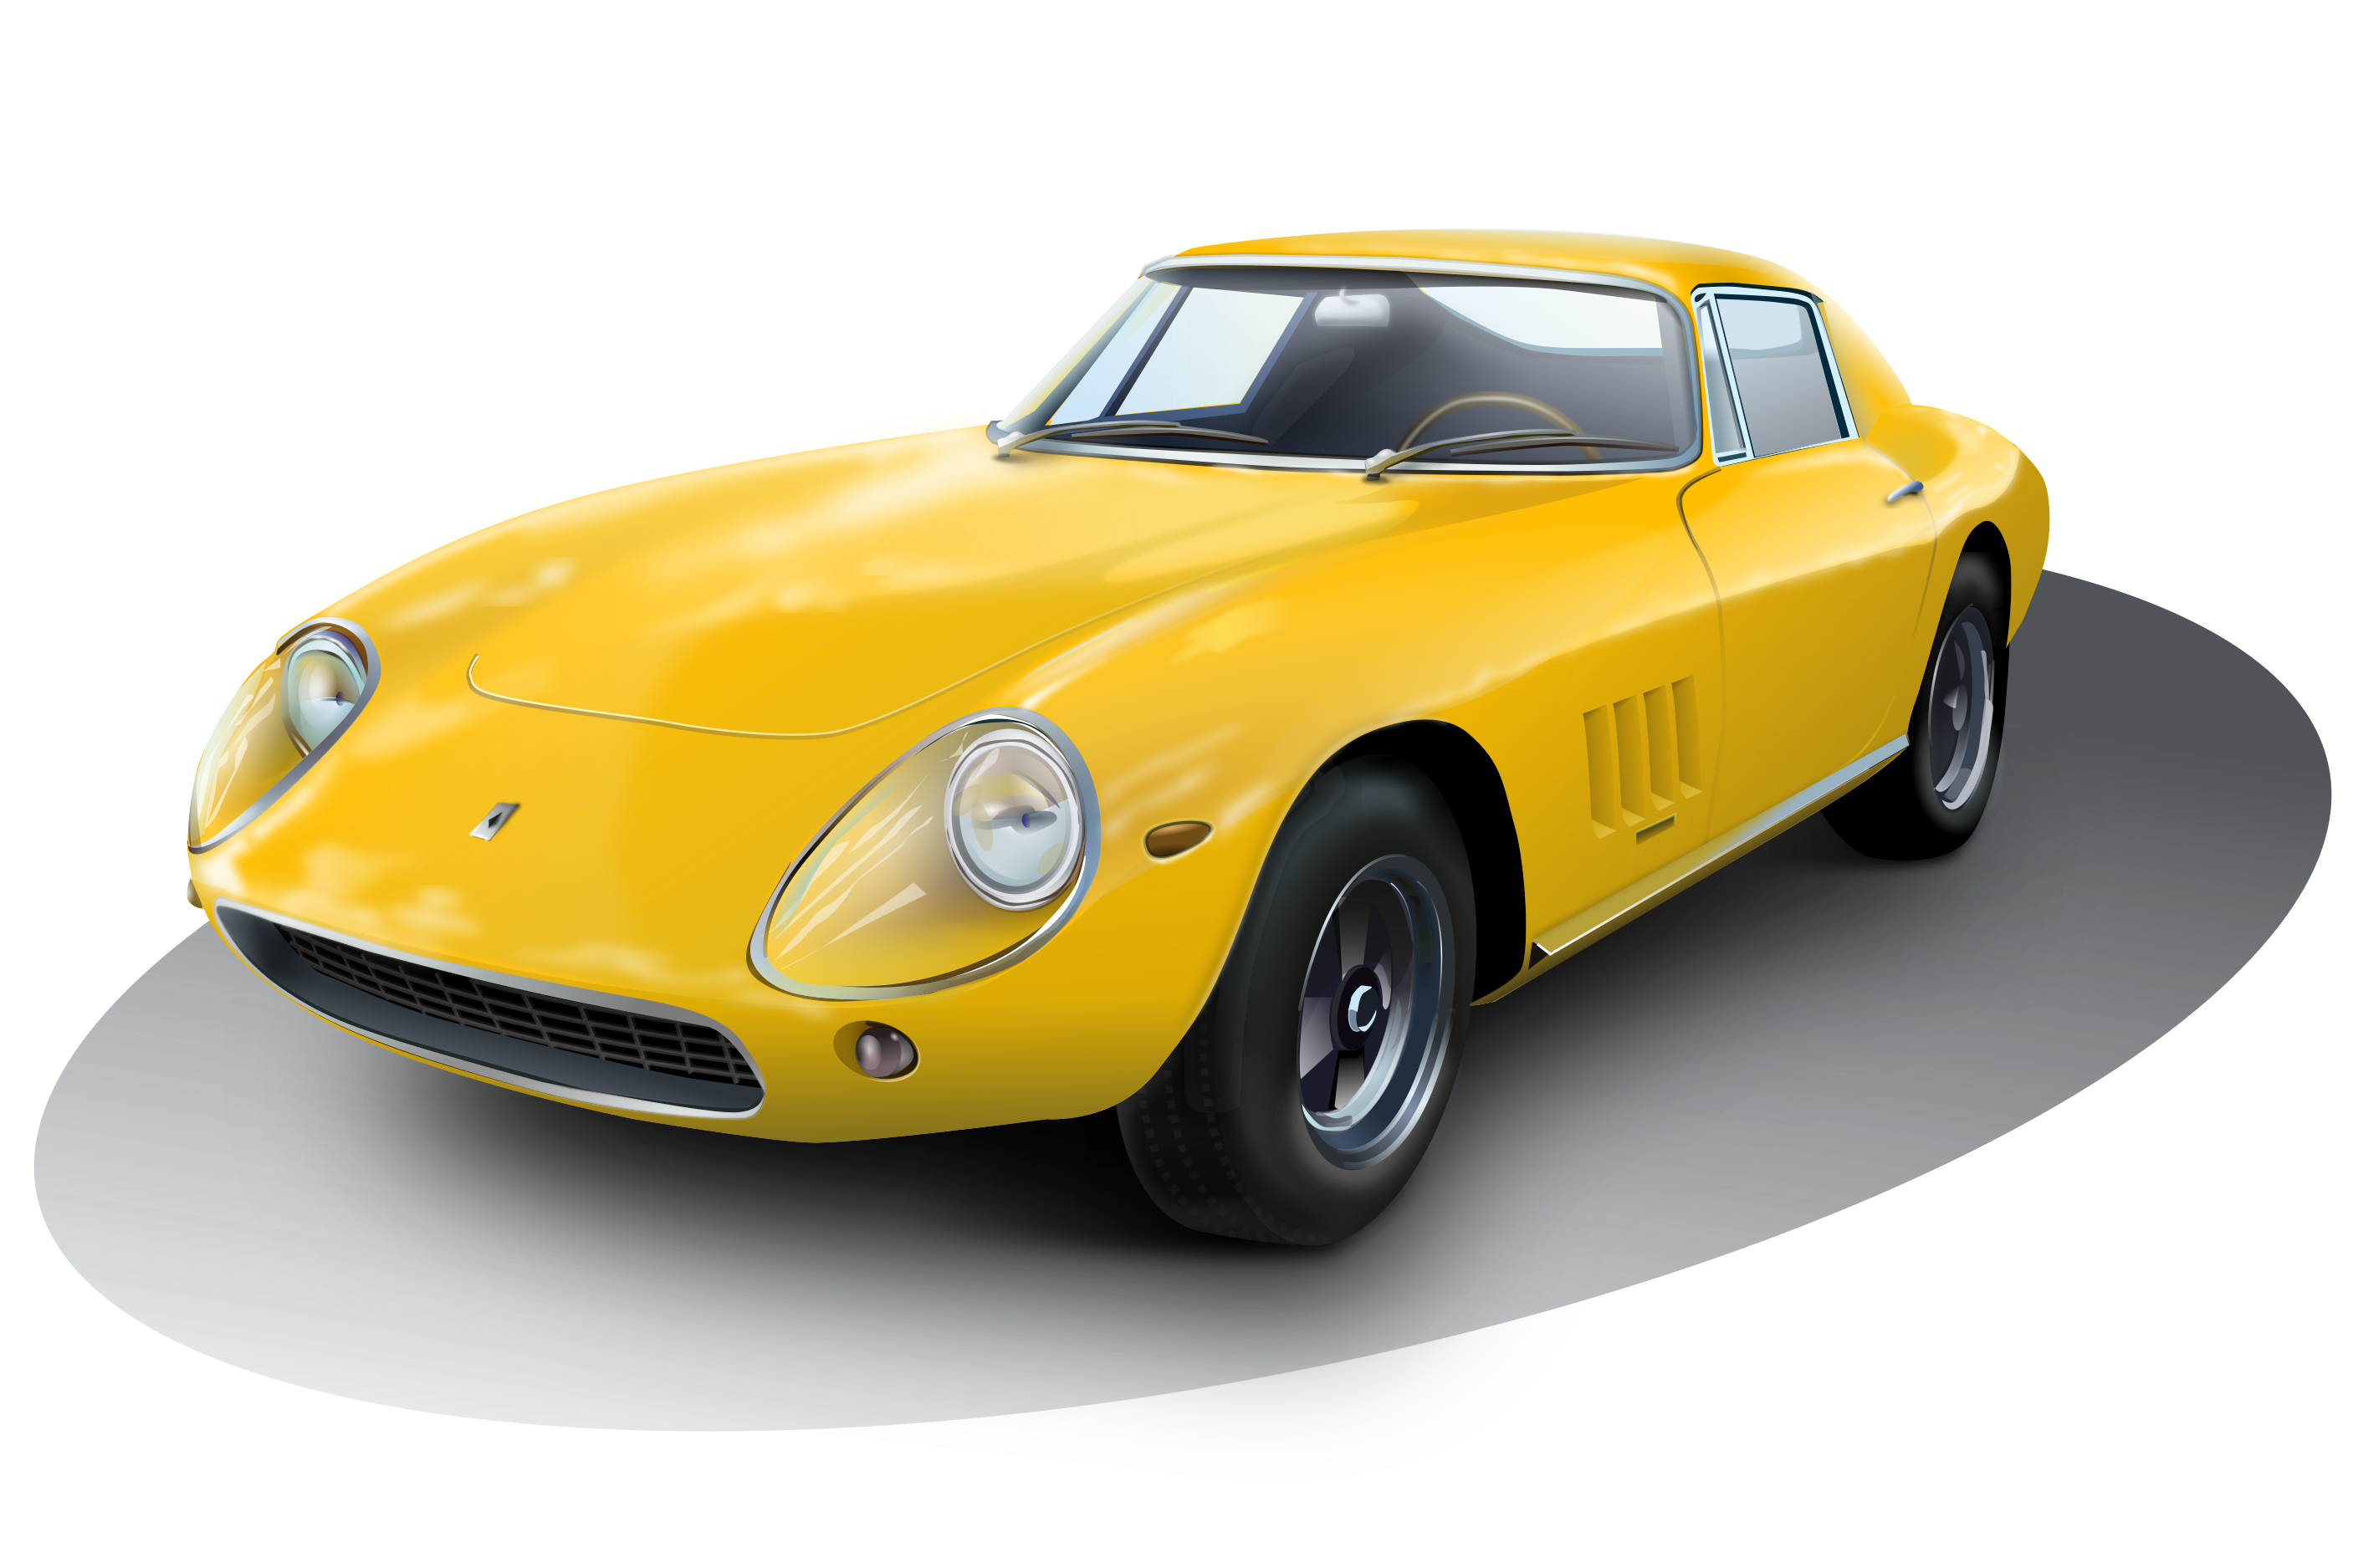
\includegraphics[scale=0.1]{Documeto/1-ElementosTextuais/1-Desenvolvimento/imagens-atividade1/car.png}

    \fonteElementoGrafico{Fornecido pelo Professor}
    
\end{figure}

\begin{figure}[h!]
    \centering
    \caption{Carro no formato SVG}
    \label{fig:carro_SVG}
    
    \includesvg[scale=0.1]{Documeto/1-ElementosTextuais/1-Desenvolvimento/imagens-atividade1/NewTux.svg}

    \fonteElementoGrafico{Fornecido pelo Professor}
    
\end{figure}

\hspace{1.5 cm} Escolheu-se essa imagem, pois, ela possui mais detalhes, o que a torna melhor para fazer esse tipo de comparação. Após converter a imagem para PNG já pode ser observado uma diferença, o tamanho da imagem aumentou quase 3,5$\times$. Depois, apenas as diferenças já explicitadas, a questão da perda de qualidade ao realizar o zoom. Para melhor exemplificar isso, seguem as Imagens \ref{fig:farol_carro_svg} e \ref{fig:farol_carro_png}.

\begin{figure}[h!]
    \centering
    \caption[Caption for LOF]{Farol do carro em SVG, zoom 500\% \footnotemark}
    \label{fig:farol_carro_svg}
    
    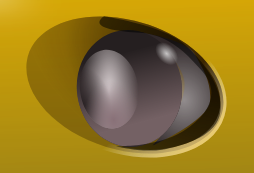
\includegraphics[scale=0.7]{Documeto/1-ElementosTextuais/1-Desenvolvimento/imagens-atividade1/farol_car_svg.png}

    \fonteElementoGrafico{Fornecido pelo Professor}
    
\end{figure}
\footnotetext{Zoom renderizado no navegador \textit{Firefox}}

\begin{figure}[h!]
    \centering
    \caption[Caption for LOF]{Farol do carro em png, zoom 500\%\footnotemark}
    \label{fig:farol_carro_png}
    
    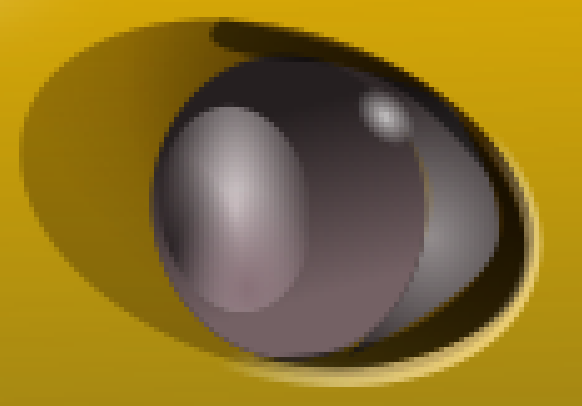
\includegraphics[scale=0.3]{Documeto/1-ElementosTextuais/1-Desenvolvimento/imagens-atividade1/farol_car_png.png}

    \fonteElementoGrafico{Fornecido pelo Professor}
    
\end{figure}
\footnotetext{Zoom renderizado pelo aplicativo \textit{Photoshop}CS5 (obviamente obtido legalmente). Escolhemos esse \textit{software} para evitar filtros que outros aplicativos possam vir a utilizar ao dar zoom.}